\documentclass[twocolumn]{article}
\usepackage{cenum}
\usepackage{paralist}
\usepackage{graphicx}
\usepackage{pictex}
\usepackage[letterpaper,margin=1in]{geometry}
\usepackage{hyperref}
\usepackage[backend=biber,
  natbib=true,
  style=ext-numeric-comp,
  sorting=nyt]{biblatex}
\DeclareFieldFormat % Titles in sentence case
  [article,inbook,incollection,inproceedings,patent,thesis,unpublished]
  {titlecase:title}{\MakeSentenceCase*{#1}}
\renewbibmacro{in:}{ % Don't use "In:" before journal names.  
  \ifentrytype{article}{}{\printtext{\bibstring{in}\intitlepunct}}}  
\addbibresource{defs.bib}
\addbibresource{tree.bib}
\addbibresource{arrunpub.bib}
\newcommand{\G}{\mathcal{G}}
\newcommand{\Het}{\mathcal{H}}
%\setlength{\topmargin}{0mm} % ouzel
%\setlength{\topmargin}{-1in} % sewall
\begin{document}
\title{Study Guide for Human Evolutionary Genetics}
\author{Alan R. Rogers}
\date{\today}
\maketitle

\section{Python}
Here is an example of the sort of question that we plan to ask:
\begin{cenum}
\item
Write down the output that would be produced by the following
snippet of Python code.
\begin{verbatim}
s = 0
for i in range(3):
    s += i*i

print(s)
\end{verbatim}
\end{cenum}
We would expect to see something like this as an answer:
\begin{verbatim}
Program prints "5".
\end{verbatim}
You only need to know about Python constructs that have been used in
the course, either in JEPy or in one of the labs.  We went through the
code in those projects and made a series of short snippets like the
one above.  Here are a few more, just to give you the flavor:
\begin{cenum}

\item
\begin{verbatim}
print("a %s b %d:%3.1f" % ("hey",12,1.2))
\end{verbatim}

\item
\begin{verbatim}
def f(x, y):
    return x*y

print(f(3,2))
\end{verbatim}

\item
\begin{verbatim}
x = 5

print("%d %s" % (x, x*"*"))
\end{verbatim}

\item
Here's one that often comes in handy when doing
calculations with gene genealogies:
\begin{verbatim}
print(sum([1/i for i in range(1,3)]))
\end{verbatim}
This last snippet is the easy way to calculate $\sum_{i=1}^2 1/i$.

\item
\begin{verbatim}
from random import random
samp_size = 100000000
n = 0
for i in range(samp_size):
    if random() < 0.7:
        n += 1

p = n/samp_size
print(p)
\end{verbatim}
\end{cenum}
The last snippet above is the longest one in our list.

\section{Probability}
\begin{cenum}
 \item Make a table showing the relative frequencies of the
   values in these data: [A, A, T, A, G].

\item In his urn experiment, Kerrich drew two balls from an urn
  \emph{without} replacement. Imagine a version of experiment in which
  each trial begins with 5 red balls and 3 black ones.  What is the
  probability that, in a single trial, both of the balls drawn are
  red?

\item Here is the probability distribution of two variables, $X$ and
  $Y$:
\begin{center}
\begin{tabular}{ccc}
$X$ & $Y$ & $\Pr[X, Y]$\\
\hline
0   &  0  & 0.2\\
0   &  1  & 0.2\\
1   &  0  & 0.1\\
1   &  1  & 0.5\\
\hline
\end{tabular}
\end{center}
What are $E[X]$, $E[Y]$, Var$[X]$, Var$[Y]$, Cov$[X,Y]$, $E[XY]$,
and $E[XY^2]$.

\item Be able to manipulate the properties of expectations listed at
  the bottom of the first column of page~6, in JEPr.  We'll ask you
  for things like $E[4X]$, $E[Y/2]$, and $E[X+Y]$.  You should be able
  to get such answers quickly, using the expectations you calculated
  in the previous item.

\item An urn contains 40 black balls and 60 red balls.  You choose a
  ball at random, put it back, and choose another at random.  What are
  the possible outcomes and their probabilities?

\item In a toss of two fair dice, one red and one black, what is the
  probability of observing a red~4 \emph{or} a black~5?

\item You toss a fair coin three times, receive \$1 for each head and
  nothing for tails.  Let $X$ represent the total number of dollars
  you receive on all three tosses.  What is the probability
  distribution of $X$?  (In other words, what are the possible values
  of $X$ and their probabilities.)

\item Suppose that, in a class of 40 students, 20 are
  women. If we choose a student at random from the class, what is the
  probability that this student is a woman?

\item If we choose 2 students from this class at random \emph{without}
  replacement, what is the probability that both are women?

\item Now you select 3 students at random \emph{with} replacement. The
  number of men in this sample is a random variable, which may equal
  0, 1, 2, or 3. What is the probability distribution of this random
  variable? (You may answer either by listing the probability of each
  outcome or by writing down a formula. Don't bother with the
  calculator.)

\item JEPr gives three formulas for the variance: $E[(X - E(X))^2]$,
  $E[X^2] - E[X]^2$, and $E[X(X - E[X])]$. Be able to calculate a
  variance using all three.

\item The preceding item is about the variance as an expected
  value. But we also calculate variances from data, and in that case
  the variance is a statistic rather than an expected value. These are
  distinct quantities, even though we use the same word for them. Make
  sure you understand the difference between a statistic and an
  expected value, and make sure you can calculate either sort of
  variance.

\item JEPr also gives three formulas for the covariance: $E[(X -
  E(X))(Y-E[Y])]$, $E[XY] - E[X]E[Y]$, and $E[X(Y - E[Y])]$. Be
  familiar with these too, both as statistics and as expected values.

\item JEPr discussed the following probability distributions:
  (1)~binomial, (2)~Bernoulli, (3)~Poisson, (4)~uniform,
  (5)~exponential, and (6)~normal. You're expected to know the mean,
  variance, and distribution function of each distribution.

\item Under what cirumstances would each distribution be plausible?
  For example, which distribution would you use to model the number of
  clicks emitted by a Geiger counter during some fixed interval of
  time? Suppose you spin a bottlecap 30 times and count the number of
  times it lands ``concave-side-up.'' Which distribution would best
  model that? Which distribution would make sense as a model of the
  length of a coalescent interval? (This last question won't make
  sense until you've read the chapter on Gene Genealogies in Rogers's
  lecture notes.)

\item For which distribution is the mean equal to the variance? For
  which is the mean equal to the standard deviation?
\end{cenum}

\section{Alleles, loci, frequencies, and heterozygosity}
\begin{cenum}
 \item Discuss the two inconsistent sets of definitions of ``locus,''
  ``gene,'' and ``allele.''
 \item A locus with two alleles is called ``biallelic.''  Data from
   such a locus may be in the form of a list of genotypes like this:
\begin{verbatim}
['AA', 'AA', 'AT', 'TA', 'TT']
\end{verbatim}
or in the form of genotype counts like this:
\begin{verbatim}
AA: 2, AT: 2, TT: 1
\end{verbatim}
Given either type of data, you should be able to calculate
(1)~genotype frequencies, (2)~allele frequencies, and (3)~genotype
frequencies expected at Hardy-Weinberg equilibrium.

\item Define genetic drift.  What events in the lives of real
  organisms contribute to drift?

\item Describe the Urn Model.  What do the balls in the urn represent?
  What do the balls drawn from the urn represent?  How does the urn
  model behave?

\item Under the influence of drift alone, heterozygosity $(\Het)$
  declines according to
\[
\Het_t = \Het_0 (1-1/2N)^t
\]
Here are a few examples of questions that we might ask about this
formula:
\begin{enumerate}
\item We might ask you to complete some step or steps of the
  derivation, so be sure you know how it goes.
\item Describe it in plain English.  What do the symbols $\Het_t$,
  $N$, and $t$ mean?
\item Genetic drift has its largest effect in small populations.  How
  is this fact reflected in the formula?
\end{enumerate}

\item At equilibrium between mutation and genetic drift, and assuming
  the infinite alleles model of mutation, the expected
   heterozygosity is
\[
\Het = \frac{4N\mu}{4N\mu + 1}
\]
There are several kinds of questions that we might ask about this
formula.  For example:
\begin{enumerate}
\item What model of mutation does this formula assume?
\item We might ask you to complete some step or steps of the
  derivation, so be sure you know how it goes.
\item What is the distinction between this formula and the formula $H
  = 2p(1-p)$ for heterozygosity at Hardy-Weinberg equilibrium?  Both
  formulas predict heterozygosity at equilibrium, so why are they
  different?  (Hint: What is meant by ``equilibrium'' in the two
  contexts?)
\item What is genetic drift, and how does it affect variation within
  and among populations?
\item Ditto for mutation?
\item How are these two effects captured by the equation above?
\item The formula above predicts the \emph{average} heterozygosity.
  Values at individual loci vary widely at any given time, from 0 up
  through levels of heterozygosity far in excess of the average.  Why?
\item Suppose that (a)~the average heterozygosity equals 0.1, and
  (b)~that $\mu=10^{-6}$.  What can you conclude about $N$?  (Assume
  that the assumptions that went into the formula above are all
  correct.)
\end{enumerate}
\end{cenum}

\section{Gene genealogies, spectrum, and mismatch distribution}
The questions that follow concern $n$ copies of a neutral DNA
sequence.  These sequences were drawn from a population of constant
size, and we are interested in their gene genealogy.
\begin{cenum}
\item How many coalescent intervals are in this gene genealogy?
\item What is the hazard of a coalescent event within the interval
  with $i$ lineages?
\item What is the expected length of this interval in generations,
  assuming that the diploid population size is $N$?
\item What is the expected age (in generations) of the last common
  ancestor?
\item What is the expected total branch length of the tree?  (In
   other words, the expected sum of the lengths of all branches.)
\item What is the expected number of segregating sites, assuming that
  there are $L$ sites, and that the mutation rate is $u$ per site per
  generation?
\item What are the expected values of $\pi$, the mean pairwise
   difference per site, and $\Pi$, the mean pairwise difference per
   sequence, using the same assumptions?
\end{cenum}
Finally, some general questions:
\begin{cenum}
\item
We have introduced a variety of statistics for measuring genetic
variation: $H$, $\pi$, $\Pi$, and $S$.  How does population size
affect the expected values of these quantities?
\item \emph{Why} does population size affect measures of genetic
  variation?  (We are expecting prose here, not formulas.)
\item
  Coalescent theory predicts that, if one population is twice as large as
  another, it should have much more heterozygosity. Is real data
  consistent with this prediction?  Why or why not?
\item
  The expected number, $S$, of segregating sites (Eqn.~5.4 of
  \emph{Lecture Notes on Gene Genealogies}) is proportional to
  population size. Thus, a population twice as large should have twice
  as many segregating sites, given samples of equal size.
  What if the populations were of equal size, but one sample was twice
  as large as the other? Would the expected number of segregating
  sites double if the sample size $K$ were twice as large? (Hint:
  calculate $\sum_{i=1}^{K-1}1/i$ for $K=2,3,4,5$. Here's how:
  \verb|sum([1.i for i in range(1,6)])|.)
\item
Theory predicts that the values of $\pi$ and $S/\sum_{i=1}^{K-1}1/i$
should be similar, because both of these estimate the same parameter.
Yet this was not true of the human data that we discussed in
class. What might account for this discrepancy?
\item Why are coalescent intervals longer near the root of the
tree? (Answer in words, not in formulas.)
\item
Why do large populations have more genetic variation than small ones?
(Answer in words, not in formulas.)

\item
How are the sizes and shapes of gene genealogies affected when the
population size, $N$, increases?  (Assume selective neutrality.)

\item
  Be able to calculate the site frequency spectrum and the mismatch
  distribution from data (for small, simple data sets). 
\item
How do they respond to changes of population size (as in the previous
section)?
\end{cenum}

\section{Neutral theory of molecular evolution}
The ``neutral theory'' is a set of ideas that explain why inferred
rates of molecular evolution tend to be similar for a given gene or
gene region, especially in closely related species.  To illustrate
this pattern we considered the mitochondrial phylogeny of a modern
human, a Neanderthal, a chimpanzee and a gorilla, as summarized in
this slide from the neutral-theory lecture.

The tree was drawn  by a method that allows the branch lengths to vary
with the number of nucleotide substitutions (mutations) that are
inferred to have occurred on each branch.  The tip of the gorilla
branch (br 1 + br 2, g) was aligned arbitrarily with the tip of the
modern human branch (br 4 + br 6, m).  The chimp branch (br 3, c) is
not constrained by that aesthetic choice, yet its tip aligns very
closely with those of the modern and Neanderthal humans, showing that
its mitochondrial genome has evolved at a very similar rate, following
separation of the chimp and human lineages around 6 million years ago.

\begin{figure}
  \centering
  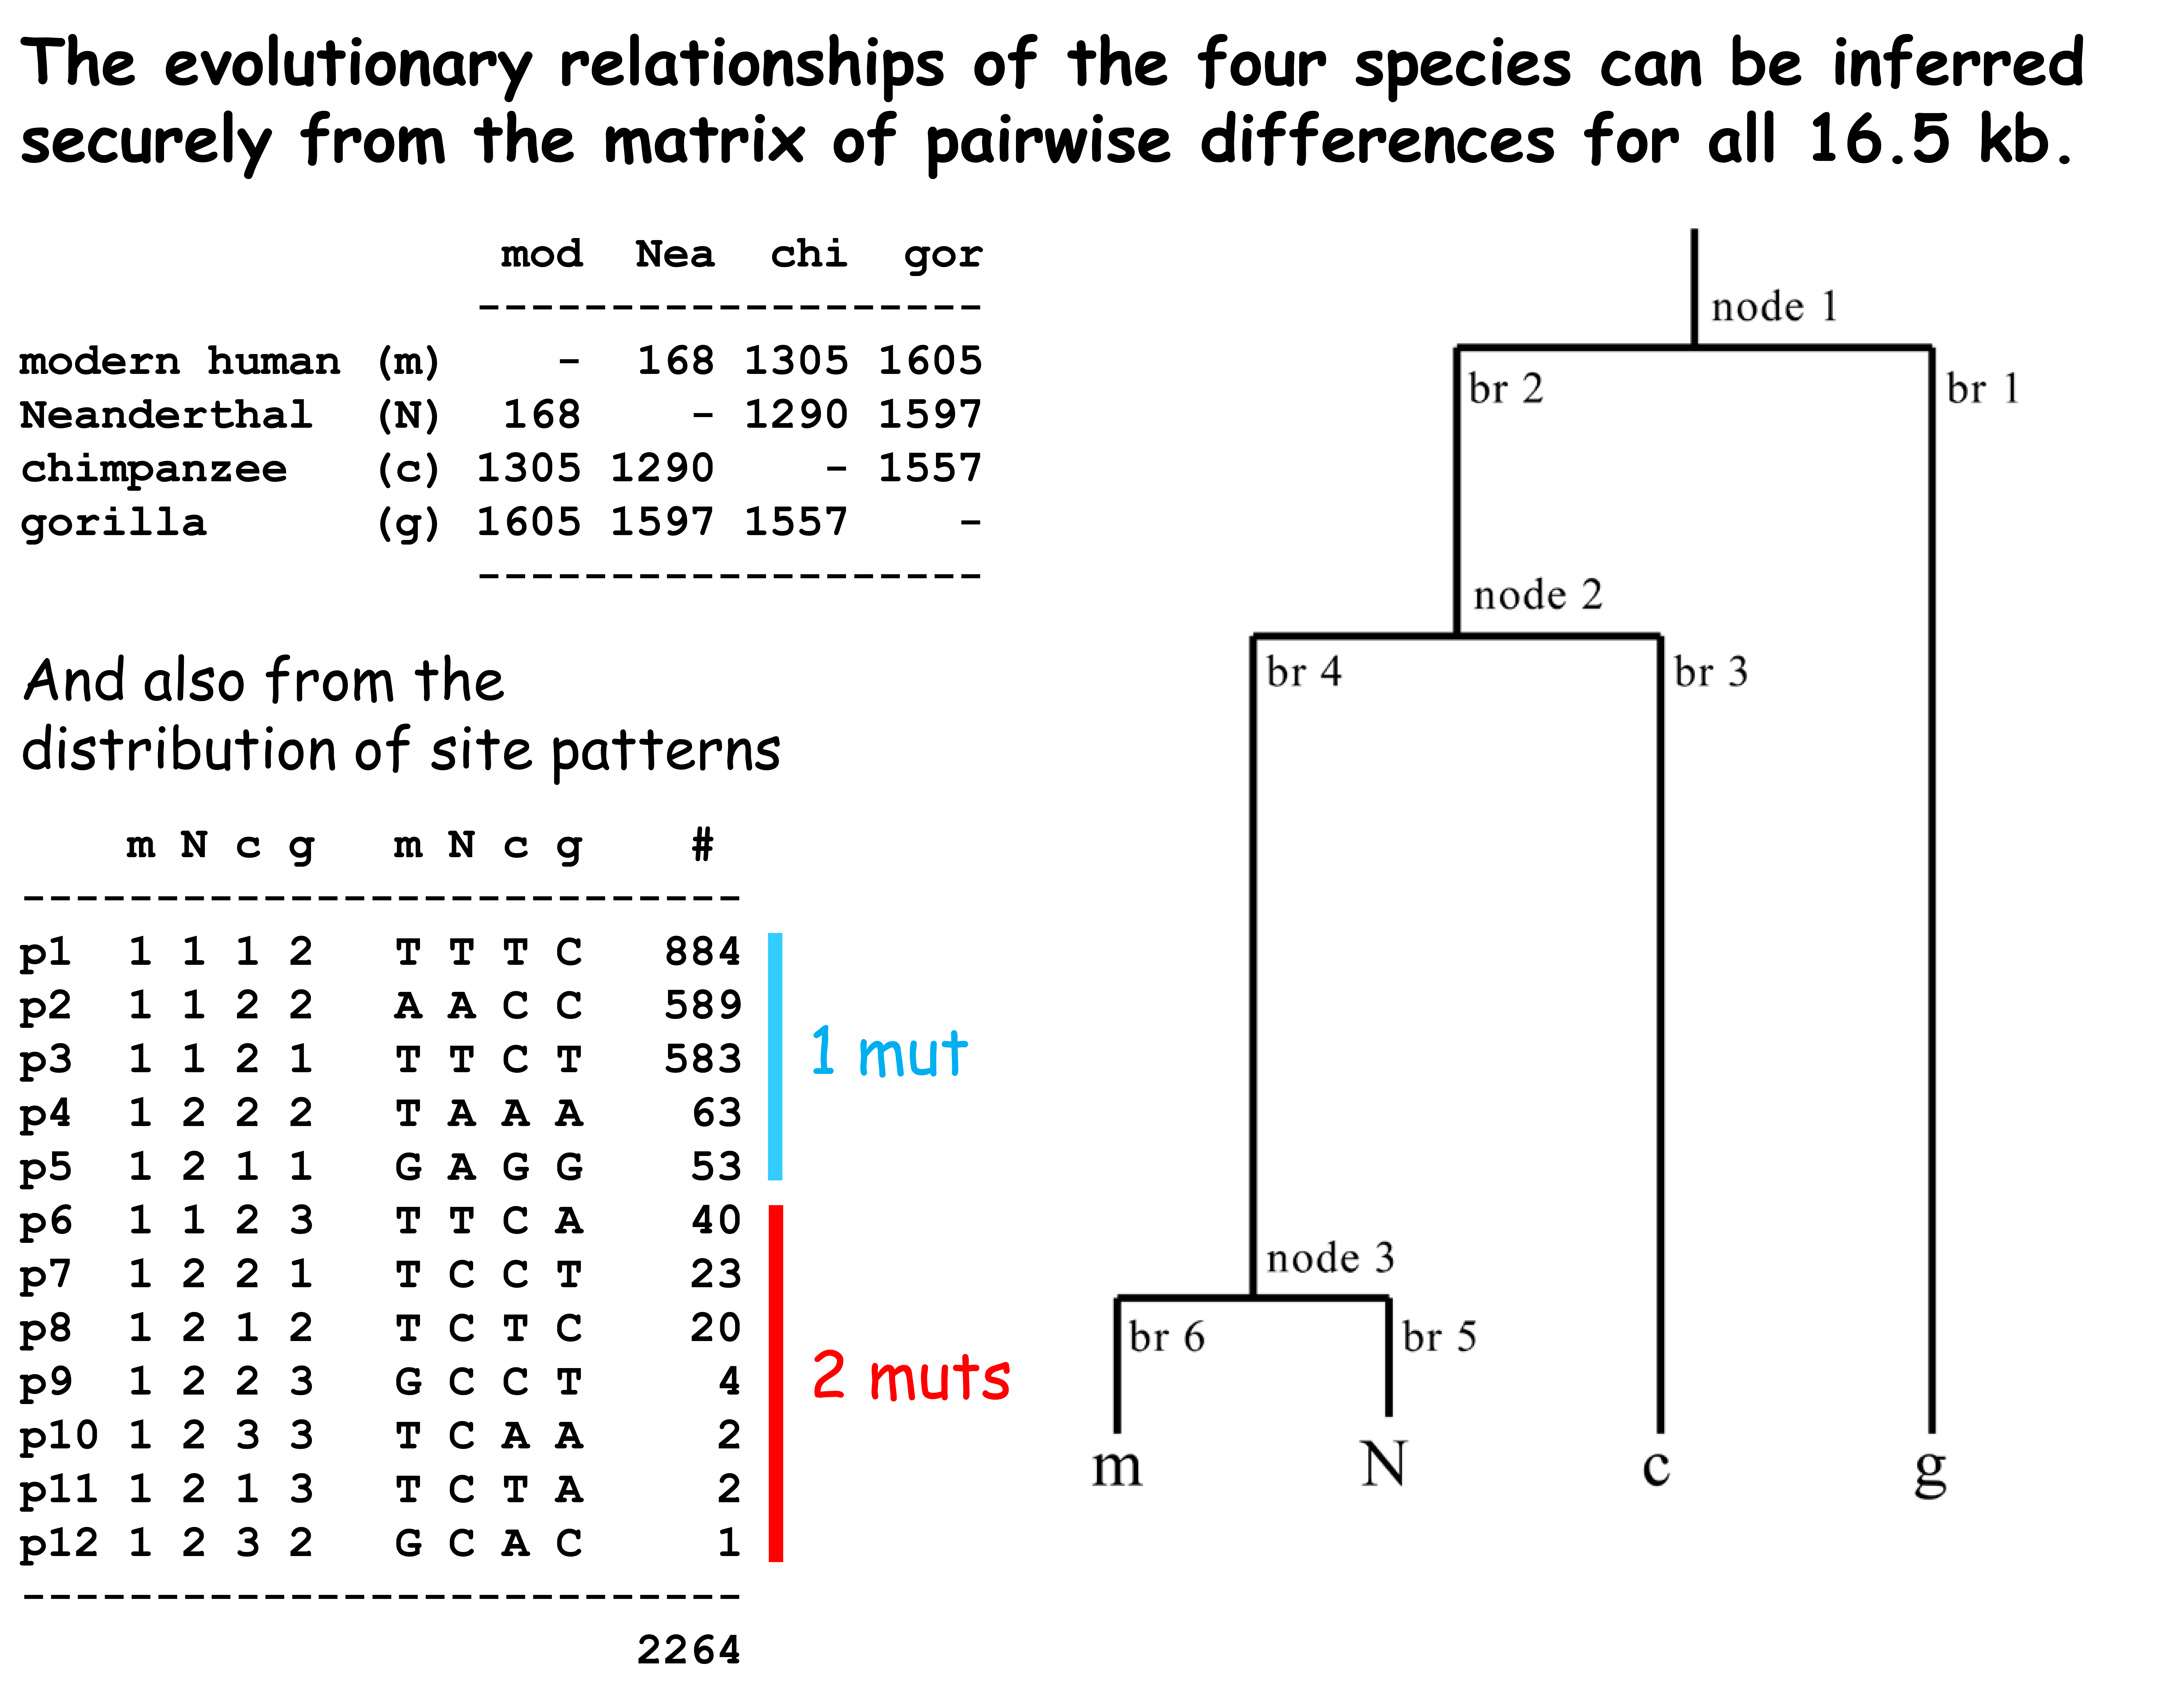
\includegraphics[width=\columnwidth]{Neutral_Theory_2022_slide_5.jpg}
\end{figure}

In the table of site patterns, the nucleotide state in the modern
human sequence (m) is arbitrarily represented as ``1'', whether
it's G, A, T or C.  The other allele(s) are represented as
``2'' and if necessary ``3''.  A particular instance of that
class of patterns is then shown in the second block of columns, and
the total number of that class of patterns in the last column.  Those
sum to 2264 sites that vary in the 4-sequence alignment; that's
roughly 14\%, implying that 86\% don't vary.
\begin{cenum}
\item Why is the first pattern (P1) the most common?
\item Why are p4 and p5 the least frequent of the patterns requiring
just one mutation?  Is their difference (63 versus 53 instances)
likely to be significant (statistically and/or scientifically)?  Why
or why not?
\item Why do we say that the number of new mutations per generation at
a given site in a given population is $2N$??  What is the meaning
(definition and/or units) of each of the three terms in this product?
\item What assumptions are we making when we say that the chance of
  ultimate fixation for any such new mutation is $1/2N$?
\item How does the chance of ultimate fixation change for mutations
with deleterious effects on the organism's phenotype, and hence its
fitness?  For mutations with beneficial effects?
\item For the triplet codons within a protein-coding sequence, at which
of the three positions (1st, 2nd, 3rd) is a new mutation most likely
to be effectively neutral?  And at which of the three positions are
mutations least likely to be effectively neutral?  Please explain your
predictions.
\item This question and the next one make use of unpublished
  mitochondrial genome sequences for six individual right whales.  The
  13 protein-coding genes taken together contain a total of 11,379
  nucleotide positions (3,793 codons).  280 codons are variable,
  meaning that at least one of the whales has at least one nucleotide
  that differs in state from the others at that position.  There are
  55 variable first positions, 13 variable second positions, and 218
  variable third positions.  (These numbers add up to more than 280
  because six of the codons vary at two different positions---either
  first and second, or first and third.)  Is this pattern consistent
  with neutral-theory expectations?  What does it imply
  (quantitatively and/or qualitatively) about the way natural
  selection really does act on typical mutations at the three codon
  positions?
\item The six right whales represent three distinct geographic
populations that are thought to have separated roughly 2-3 million
years ago (Mya): the southern right whale (Eubalaena australis), the
North Atlantic right whale (E. glacialis), and the North Pacific right
whale (E. japonica).  Their closest living relative is the bowhead
whale (Balaena mysticetus, formerly called the ``Greenland right
whale''), from which their ancestral lineage separated around 6 Mya.
Use the pairwise difference matrices below to infer the mitochondrial
phylogeny for all seven whales, using the simple clustering method
called UPGMA (https://en.wikipedia.org/wiki/UPGMA).  First make the
tree implied by the differences at third codon positions only, and
then make the tree implied by the differences at first and second
positions only.
\end{cenum}
In which tree do you have more confidence, and why?  Note that the
UPGMA method assumes a ``clock-like'' accumulation of differences
with time.  The two kinds of sites clearly have very different clock
rates, but if we recalibrate by assuming that the separation between
the bowhead and right-whale lineages occurred around 6 Mya, do both
trees give similar dates for the splits among the three right-whale
species?

Would you expect to get the best result by combining all of the data
(that is, by adding the two distance matrices)?  Feel free to give
that a try.  In any case, please explain your reasoning.

\begin{table}
{\small\renewcommand{\tabcolsep}{3pt}\begin{tabular}{lrrrrrrr}
\multicolumn{8}{l}{\normalsize Raw distance matrix, position 3}\\[3pt]
 & Bmy & Eau1 & Eau2 & Egl1 & Egl2 & Eja1 & Eja2\\ \cline{2-8}
Bmy & 0 & 452 & 458 & 450 & 453 & 467 & 467\\
Eau1 & 452 & 0 & 36 & 108 & 113 & 130 & 130\\
Eau2 & 458 & 36 & 0 & 104 & 109 & 134 & 132\\
Egl1 & 450 & 108 & 104 & 0 & 9 & 130 & 128\\
Egl2 & 453 & 113 & 109 & 9 & 0 & 133 & 131\\
Eja1 & 467 & 130 & 134 & 130 & 133 & 0 & 34\\
Eja2 & 467 & 130 & 132 & 128 & 131 & 34 & 0\\
\hline
\\[10pt]
\multicolumn{8}{l}{\normalsize Raw distance matrix, positions 1--2}\\[3pt]
 & Bmy & Eau1 & Eau2 & Egl1 & Egl2 & Eja1 & Eja2\\ \cline{2-8}
Bmy & 0 & 115 & 118 & 132 & 134 & 119 & 120\\
Eau1 & 115 & 0 & 13 & 35 & 35 & 26 & 27\\
Eau2 & 118 & 13 & 0 & 40 & 40 & 31 & 30\\
Egl1 & 132 & 35 & 40 & 0 & 6 & 45 & 46\\
Egl2 & 134 & 35 & 40 & 6 & 0 & 45 & 46\\
Eja1 & 119 & 26 & 31 & 45 & 45 & 0 & 13\\
Eja2 & 120 & 27 & 30 & 46 & 46 & 13 & 0\\
\hline
\end{tabular}}
\end{table}  

\section{Selection}
\begin{cenum}
\item
Assuming fixed, constant fitnesses for the three genotypes at a biallelic
diploid locus, what is the \emph{mean fitness} of the population?

\item
What are the \emph{marginal fitnesses} of the two alleles?

\item
What is next generation's expected allele frequency ($p'$ or $q'$), as a
function of these quantities?

\item How can an observed rate of allele-frequency change be used to
  estimate the relative fitnesses of two alleles (for example, $s$, if
  we know the value of $h$)?  This was the subject of some homework
  problems. 

\item Selection is slow when a recessive allele is rare. Why?

\item Selection is slow when a dominant allele is common. Why?

\item A rare allele tends to spread if its heterozygote is fitter than
  the common homozygote. Why? Why doesn't the fitness of the rare
  homozygote matter?

\item What stable equilibria exist if $w_{11} > w_{12} > w_{22}$?  

\item What stable equilibria exist if $w_{11} < w_{12} > w_{22}$?

\item When the heterozygote has highest fitness, and the two
  homozygotes differ in fitness, which allele is most common at the
  stable equilibrium?

\item What stable equilibria exist if $w_{11} > w_{12} < w_{22}$?

\item Selection pushes allele frequency in the direction that
  increases the mean fitness of the population. Consequently, stable
  equilibria occur at peaks in the graph of mean fitness against
  allele frequency.

\item How long does it take for an advantageous allele to sweep from
  frequency 0.01 to 0.99 in a large population, assuming that allelic
  effects are additive (no dominance) and that the fitness of the
  favored homozygote is 1.018 times that of the other homozygote?

  \bigskip

  \emph{Answer:} The coefficient of selection is $s = 0.018$, so the
  answer is $18/s = 1000$ generations.
\end{cenum}

\section{Interactions of mutation, drift and selection}
\begin{cenum}
\item
What is the fixation probability for a newly arisen neutral mutation?

\item What is the \emph{approximate} fixation probability for a newly
  arisen mutation that is favored by a selection coefficient of $s$
  (relative fitness $1+s$) in the homozygous state, and $s/2$ in the
  heterozygous state?  Does the population size $N$ affect our answer?
  If so, how?
\item
What is the expected rate at which adaptive mutations will fix within
a species, given a certain population size $(N)$, selective advantage
$(s)$, and genome-wide rate of mutation ($U$) to alleles with
advantages of about that size?

% \item Inbreeding depression might be caused either by partially
%   recessive deleterious alleles that are relatively abundant
%   (everyone carries many of them) or by overdominant alleles (ones
%   beneficial only in heterozygotes).  Does the analysis of Crow and
%   Morton (see lecture notes and text) allow us to choose between
%   these hypotheses?  Explain.

\item
Why are most deleterious alleles (the ones segregating at appreciable
frequencies) at least partly recessive?
\item
Under what conditions will a deleterious (harmful) mutation have nearly as good
a chance of fixing as a neutral mutation?
\item
Do we expect more adaptive evolution in large or small populations? Explain.
\item Do we expect to find more or fewer harmful mutations segregating
  in a selfing plant species (for example, rice) than in a
  predominantly outbreeding relative?  Explain.
\end{cenum}

\section{Multiple loci}
\begin{cenum}
\item Be familiar with Gillespie's notation ($x_1$, $x_2$, $x_3$, and
  $x_4$) for frequencies of two-locus haplotypes, where each locus has
  two alleles. Remember that $p_A = x_1 + x_2$ and $p_B =
  x_2+x_4$. (Sec.~4.1, p.~102 of Gillespie.) Also, $D = x_1 x_4 - x_2
  x_3$.

%\item Under random mating, what are the frequencies of all possible
%  two-locus genotypes (AB/AB, AB/aB, and so on)? You should be able to
%  answer this using either of the two notations: either in terms of
%  $x_1$, $x_2$, $x_3$, and $x_4$, or in terms of $p_A$, $p_B$, and
%  $D$.

\item If we gave you the frequencies of these four gamete types, you
  should be able to give us the allele frequencies and $D$ (the
  coefficient of linkage disequilibrium). Or the other way around.

\item
What are the relationships among these two measures of linkage
disequilibrium: $D$ and $r_H$?  (Here, $r_H$ refers to the gametic
correlation between two loci.  We used this symbol in the lab manual.
Gillespie uses ``$r$'' for the same purpose.)
\end{cenum}

%Suppose that in an initial generation, $x_1$, $x_2$, $x_3$, and $x_4$,
%are equal to 0.2, 0.3, 0.4, and 0.1 and that the recombination rate is
%$c=1/10$.

\begin{cenum}
%\item What are $p_A$, $p_B$, and $D$ in this initial generation?

%\item What are the expected values of these quantities after
%  1~generation? After 100~generations?

%\item In lecture, Rogers explained that (a)~selection does not
%  generate linkage disequilibrium (LD), but nonetheless (b)~LD is
%  useful in detecting ongoing selective sweeps.  Why is this not a
%  contradiction? (See ``Why linkage disequilibrium helps us find
%  selective sweeps'' on the class website.)

\item Locus $B$ has two alleles: $B_1$ (with frequency $p_1$), and
$B_2$ (with frequency $1-p_1$).  A new mutation arises at a linked
locus, $A$.  What is the probability that this mutant chromosome
carries allele $B_1$?

\item Mammalian genomes (including ours) are typically about 3~Gbp
  (billion base pairs) in length, but most of that DNA is
  non-functional ``junk'' that doesn't code for proteins or structural
  RNAs, and doesn't play any important role in the regulation of gene
  expression.  Some of these neutral nucleotides are close to
  functional genes, and others are far away.  How would you expect
  proximity to functional genes to affect the variability of these
  neutral nucleotides?  Are the ones near genes more likely to be
  polymorphic, or less?

%\item
%In Gillespie's standard setup, there are four gamete types $A_1B_1$,
%$A_1B_2$, $A_2B_1$, and $A_2B_2$, with frequencies $x_1$, $x_2$,
%$x_3$, and $x_4$.  Suppose that, in generation~1, half the gametes are
%$A_1B_1$ and half are $A_2B_2$.
%\begin{enumerate}
%\item What is $D$?
%\item Now assume that selection operates at the gamete stage, that
%  alleles $B_1$ and $B_2$ are neutral, that allele $A_1$ has fitness
%  $1+s$ relative to $A_2$, and that the recombination rate is $c=1/3$.
%  What are the expected values of the four gamete frequencies in the
%  following generation? (Hint: Use the formula for selection at the
%  gamete stage, which we gave in lecture.)
%\end{enumerate}

\item When an allele sweeps to fixation at locus $A$, (a)~what happens to
the frequencies of neutral alleles at linked loci?  (b)~What happens
to $D$?

\item Linkage disequilibrium is often obvious in tables of DNA
sequence (or SNP) data.  For examples, see our slides.
Be able to recognize it when you see it.

\item What is genetic draft?  What problem was it invented to explain?
How is it affected by the following parameters: $N$, $\mu$, $c$
(recombination rate)?
\end{cenum}

\section{Inbreeding}
\begin{cenum}
\item What is inbreeding depression, and what causes it?

\item The inbreeding coefficient $(F)$ can be interpreted as a measure
  of either
\begin{inparaenum}
\item departure from Hardy-Weinberg genotype frequencies,
\item inbreeding within a pedigree,
\item inbreeding between random individuals within a
  population, or
\item the effect of genetic drift.
\end{inparaenum}
In the first sense, it is the proportional reduction in heterozygosity
relative to that expected at Hardy-Weinberg equilibrium. In the second
sense, it is the probability of identity by descent (IBD) relative to the
oldest generation in the pedigree. Senses 3--4 are like~2 but refer to
a random individual within a population rather than to a specific
individual. 

\item
Be able to express the frequencies of the three genotypes at a
biallelic locus ($P_{11}$, $P_{12}$, and $P_{22}$) in terms of $p_1$
and $F$.

\item The formulas in the preceding question can be used to represent
  the effect of non-random mating in a single generation, or the
  effect of drift across many generations. How do the interpretations
  of $p$ and $F$ change in these two situations? (Hint: your answer
  should involve the ``reference generation.'')

%\item
%Genotype frequencies can be written in two algebraically equivalent
%forms. For example, $P_{AA}$ can be written either as $p^2 + p(1-p)F$
%or as $Fp + (1-F)p^2$. Be familiar with both forms.

\item
What is the connection between inbreeding and genetic drift?

\item
Consider the following genealogy:
\begin{center}
\begin{minipage}{1cm}
\begin{verbatim}
F    G
|\  /|
| \/ |
| /\ |
|/  \|
D    E
|    |
|    |
|    |
|    |
B    C
 \  /
  \/
   A
\end{verbatim}
\end{minipage}
\end{center}
In this genealogy, A is the offspring of B and C, which are the
offspring of D and E, and so on.
\begin{inparaenum}
\item The two genes that united to form A may be identical by descent (IBD)
  from which ancestors?
\item For each of these ancestors, calculate the probability of
  IBD.  (In other words, calculate the contribution of each loop in
  the pedigree to A's inbreeding coefficient.
\item What is A's inbreeding coefficient?
\item What is the coefficient of kinship of D and C?
\item In what way, if any, do we expect A to differ \emph{genetically}
  from typical (outbred) members of the population?  Explain briefly.
\item In what way(s) might we expect A to differ \emph{phenotypically}
from outbred members of the population?  Explain briefly.
\end{inparaenum}

\noindent\textbf{Answers}:
\begin{inparaenum}
\item F, and G;
\item 1/32 for F or G;
\item $F = 2 \times 1/32 = 1/16$;
\item $f_{DC} = 1/8$.
\item Individual A will be heterozygous at fewer loci than will the average
member of the population, because there is an appreciable probability
that the gene copies he inherited from his two parents were identical
by descent from a common ancestor (F or G).
\item Individual A is likely to be somewhat shorter than the average
individual and somewhat less healthy, because he will have fewer loci
that exhibit heterozygote advantage and more that are homozygous for
recessive deleterious alleles.
\end{inparaenum}

\begin{figure}
{\centering% Darwin-Wedgewood Genealogy
\mbox{\beginpicture
\setcoordinatesystem units <0.85cm,1cm>
\setplotarea x from -1 to 7, y from 0 to 6
%\setdots
%\axis invisible bottom ticks andacross numbered from -1 to 7 by 1 /
%\axis invisible left ticks andacross numbered from 0 to 6 by 1 /
%\setsolid
\setplotsymbol ({\footnotesize .})
\arrow <10pt> [.2,.67] from 1 5.5 to 1 4.5
\arrow <10pt> [.2,.67] from 1 5.5 to 6 4.5
\arrow <10pt> [.2,.67] from 6 5.5 to 1 4.5
\arrow <10pt> [.2,.67] from 6 5.5 to 6 4.5
%
\arrow <10pt> [.2,.67] from 1 3.5 to 1 2.5
\arrow <10pt> [.2,.67] from 6 3.5 to 6 2.5
%
\arrow <10pt> [.2,.67] from 1 1.5 to 3.5 0.5
\arrow <10pt> [.2,.67] from 6 1.5 to 3.5 0.5
%
\put {\frame <1ex> {\sf Josiah Wedgewood}} at 1 6
\put {\frame <1ex> {\sf Sarah Wedgewood}}  at 6 6
\put {\frame <1ex> {\sf Susannah Wedgewood}} at 1 4
\put {\frame <1ex> {\sf Josiah Wedgewood II}} at 6 4
\put {\frame <1ex> {\sf Charles Darwin}} at 1 2
\put {\frame <1ex> {\sf Emma Wedgewood}} at 6 2
\put {\frame <1ex> {\sf George Darwin}} at 3.5 0
\endpicture}
\\}
\caption{Genealogy of George Darwin}
\label{fig.darwedge}
\end{figure}

\item Figure~\ref{fig.darwedge} shows the genealogy of George
  Darwin, one of Charles Darwin's sons. What is his inbreeding
  coefficient?
\end{cenum}

\section{Non-random mating}
\begin{cenum}
%\item Suppose that a population consists of several subdivisions (or
%  groups) of equal size, within each of which mating is at random.
%  The mean of group allele frequencies is 1/2 and their variance is
%  1/4.  What is the expected heterozygosity in the population as a
%  whole?  (Hint: See the Wahlund Effect, discussed in lecture and in
%  the text.)

\item What is $F_{ST}$, and what does it measure?  How does it
increase with time among a group of isolated populations, such as
those in Buri's experiment?  What equilibrium does it reach if the
effects of drift are opposed by gene flow?

%\item Suppose that we ran an experiment like Buri's---one in which
%  genetic drift was the only force at work, the effective
%  population size was constant at $N=50$ within each group, and our
%  organisms were diploid.  Unlike Buri's organisms, ours mated at
%  random.  The initial heterozygosity was $H_0 = 1/2$,
%  and we ran the experiment for 5 generations.
%  \begin{enumerate}
%\item What is the expected heterozygosity in the final (the
%  5th) generation?
%\item What is the expected value of $F_{ST}$?
%\item What is the average inbreeding coefficient of individuals in the
%  5th generation relative to the initial (the 0th) generation?
%\end{enumerate}

%\item
%Use the data in the table below to estimate $F_{ST}$.  (Hint: you only
%need the last line.)
%\begin{center}
%\begin{tabular}{lcc}
%Population & $p$ & $p^2 + q^2$\\
%\hline
%African    & 0.734 & 0.610\\
%European   & 0.496 & 0.500\\
%Australian & 0.330 & 0.558\\
%East Asian & 0.259 & 0.616\\
%\hline
%Average    & 0.455 & 0.571\\
%\end{tabular}
%\end{center}
%\begin{verbatim}
%>>> p = 0.455
%>>> gt = 1 - 2*p*(1-p)
%>>> gs = 0.571
%>>> fst = (gs-gt)/(1-gt)
%0.13499344692005213
%\end{verbatim}

\item
Among continental human populations, estimates of $F_{ST}$ are usually
close to $1/9$.  Assume that this represents an equilibrium between
migration and genetic drift under the Island Model of population
structure.  What does this imply about the number $Nm$ of migrants
between pairs of populations in each generation? \textbf{Answer:}
\[
  1/9 = \frac{1}{4Nm + 1} \Rightarrow Nm=2
\]
\end{cenum}  

\section{Human evolutionary history}
\begin{cenum}
\item What is known about the history of human population size during
  the past two million years? When was the population large? When was
  it small? How do these events relate to (a)~the expansion of
  \emph{Homo erectus} out of Africa, about 2~Ma ago, (b)~the expansion
  of modern humans out of Africa about 50~ka ago, (c)~the coldest part
  of the last ice age about 20~ka ago, and (d)~the beginning of the
  Holocene (the warm period in which we now live) about 12~ky
  ago?\footnote{To prepare for this question, look at the slide
    labeled ``PSMC estimates from autosomes'' from the lecture
    ``Population history from whole genomes.'' (You can also find this
    graph in the article by Li and Durbin.) What does the graph say
    about population size at the times listed in the question?}
\item When and where did Neanderthals live? Which modern populations
  carry DNA derived from Neanderthal ancestors? In modern Eurasians,
  what fraction of the DNA derives from Neanderthals?
\item Expect the same question about Denisovans, except that we don't
  know much about when and where they lived. (They seem to have been
  contemporaneous with Neanderthals, but probably lived in Asia,
  Indonesia, and/or New Guinea.)
\item At some loci, archaic alleles seem to have been favored by
  selection in modern populations. In which functional category (or
  categories) of gene is this beneficial effect strongest? Why might
  archaic alleles have been beneficial to modern humans at these loci?
\item At other loci, archaic alleles were selected against in modern
  humans. How do we know? Why might we expect deleterious alleles to
  have been common in archaic genomes?
\item What do we know about the ``neandersovan'' ancestors of
  Neanderthals and Denisovans? When did they separate from the lineage
  leading to modern humans? When did they split into Neanderthals and
  Denisovans? How large was their population? With whom did it
  interbreed?
\end{cenum}
Some vocabulary: The ``mesolithic'' of Europe refers to the period
after the Ice Ages but before agriculture. During this period,
Europeans lived by gathering and hunting medium-sized animals. The
following period, the ``neolithic,'' Europeans farmed and raised
domestic animals but did not yet make metal tools. After the neolithic
came the ages of copper, of bronze, and of iron.
\begin{cenum}
\item What do we know about the history of skin and eye color in
  Europe? How did these characters change from the mesolithic (say
  8000~bp) to the neolithic (say 6000~bp) to the bronze age (say
  4000~bp) to the recent period?
\item Same question, but about lactase persistence: the ability to
  digest milk sugar (lactose) beyond childhood.  
\end{cenum}

\section{Quantitative traits}
\begin{cenum}
\item What are quantitative traits?

\item Why are they often normally (or near-normally) distributed?

\item What is the phenotypic variance ($V_P$)?

  \item What are the relationships (mathematical and biological) among
    the variance components $V_P$, $V_G$, $V_A$, $V_D$ and $V_E$?

  \item What is the narrow-sense heritability ($h^2$) and why is it
    important?

  \item How can each of the variance components be estimated
    for real populations?

  \item Why do heritability estimates for one population have little
    validity for another population of the same species?  (In other
    words, why do we have to make the estimates anew, from actual
    data, to be confident of their values in a given population?)

  \item Related question: if a trait is highly heritable within each
    of two populations, why does this \emph{not} imply that the
    difference between those populations is genetic?

\item
Response to selection can be predicted either from
\begin{eqnarray*}
R &=& h^2 S, \qquad\hbox{or from}\\
\Delta x &=& V_a \beta
\end{eqnarray*}
Gillespie discusses only the first formulation. The second is covered
by \citet{Rogers:lande}, which is available on the class website. Be
familiar with both forumulations and able to manipulate them.

\item
What evidence suggests that long-term rates of quantitative trait
evolution are not limited by amounts of heritable genetic
variation?
\end{cenum}

\printbibliography

\end{document}
